%! TeX root = /Users/trustinnguyen/Downloads/Berkeley/Math/Math143/Homework/Math143Hw6/Math143Hw6.tex

\documentclass{article}
\usepackage{/Users/trustinnguyen/.mystyle/math/packages/mypackages}
\usepackage{/Users/trustinnguyen/.mystyle/math/commands/mycommands}
\usepackage{/Users/trustinnguyen/.mystyle/math/environments/article}
\graphicspath{{.images/}}

\title{Math143Hw6}
\author{Trustin Nguyen}

\begin{document}

    \maketitle

\reversemarginpar

\textbf{Exercise 1}: Practice with topology
    \begin{itemize}
        \item [(a)] Let $X$ be an algebraic set and let $\mathcal{U} = \{X \backslash Z : Z \subseteq X \text{ is an algebraic subset}\}$. Check that $\mathcal{U}$ is a topology on $X$. This is called the \textit{Zariski topology on} $X$.
            \begin{proof}
                We just need to check that the set of complements of elements of $\mathcal{U}$ define a topology based on closed sets. Let $Z_{i}$ be algebraic sets. We know that 
                    \begin{equation*}
                        \bigcap_{i = 1}^{\infty} Z_{i}
                    \end{equation*}
                is also an algebraic set. We also have that
                    \begin{equation*}
                        \bigcup_{i = 1}^{n} \mathbb{Z}_{i}
                    \end{equation*}
                form an algebraic set. So if $\mathcal{C}$ denotes the set of algebraic set, then $\mathcal{C}$ is a topology and therefore, the set of open sets, $\mathcal{U}$ is also a topology.
            \end{proof} 

        \item [(b)] Let $X$ and $Y$ be algebraic sets and let $\varphi : X \rightarrow Y$ be a morphism. Consider $X$ and $Y$ with their Zariski topology. Prove that $\varphi$ is a continuous map.
            \begin{proof}
                We know that $\varphi$ is a continuous map if the preimage of a closed set is a closed set. Since for polynomial maps between algebraic sets, we know that the preimage of an algebraic set is an algebraic set, this says that the map is continuous.
            \end{proof}

        \item [(c)] Let $Z \subseteq \mathbb{A}^{n} \cong \mathbb{C}^{n}$ be an algebraic subset. Prove that $Z \subseteq \mathbb{C}^{n}$ is closed in the classical topology on $\mathbb{C}^{n}$.
            \begin{proof}
                We know that $Z = V(f_{1}, \ldots , f_{r})$. So $Z$ is the collection of points that vanish at each $f_{i}$. Now consider the polynomial $f_{1} \cdots f_{r}$. We will show that $\{0\}$ is closed in $\mathbb{C}^{n}$ later. If we have that $\{0\}$ is closed, we know that its preimage is a closed set in the classical topology, which is just $Z$. 

                ($\{0\}$ is closed). Consider $\mathbb{C}^{n}\backslash \{(0, \ldots , 0)\}$. Then for a point $p \in \mathbb{C}^{n}$, we can choose $\varepsilon < \lVert p \rVert$ which gives us:
                    \begin{equation*}
                        \{r \in \mathbb{C}^{n} : \lVert p - r \rVert < \varepsilon\} 
                    \end{equation*}
                does not include $0$, and therefore, is an open set. So $\{0\}$ is closed.

                This generalizes to any field with a measure of distance, so in general, we have that if $Z$ is an algebraic subset of $\mathbb{A}^{n}$, then $Z$ is closed in the classical topology on $\mathbb{A}^{n}$. This also means that open sets in the Zariski topology are also open sets in the classical topology, and therefore, $\mathcal{U}$ as a Zariski topology is coarser than $\mathcal{V}$ as a classical topology because $\mathcal{U} \subseteq \mathcal{V}$ where $\mathcal{U}, \mathcal{V}$ are the sets of open sets on each topology.
            \end{proof}
    \end{itemize}

\textbf{Exercise 2}: Find the Zariski closures of the following subsets of $\mathbb{A}^{n}$. Draw a picture of the set (or at least its real points) and its closure. Justify your answer.
    \begin{itemize}
        \item [(a)] $\{(\sin{t}, \cos{t}) : t \in \mathbb{R}\} \subseteq \mathbb{A}^{2}_{\mathbb{C}}$
            \begin{proof}
                We know that $\{(\sin{t}, \cos{t} : t \in \mathbb{R})\} \subseteq V(x^{2} + y^{2} - 1)$. But $V(x^{2} + y^{2} - 1) \not\subseteq \{(\sin{t}, \cos{t}) : t \in \mathbb{R}\}$ as $(i, \sqrt{2}) \in V(x^{2} + y^{2} - 1)$. So I don't know. Here's the picture anyway:
                    \begin{center}
                        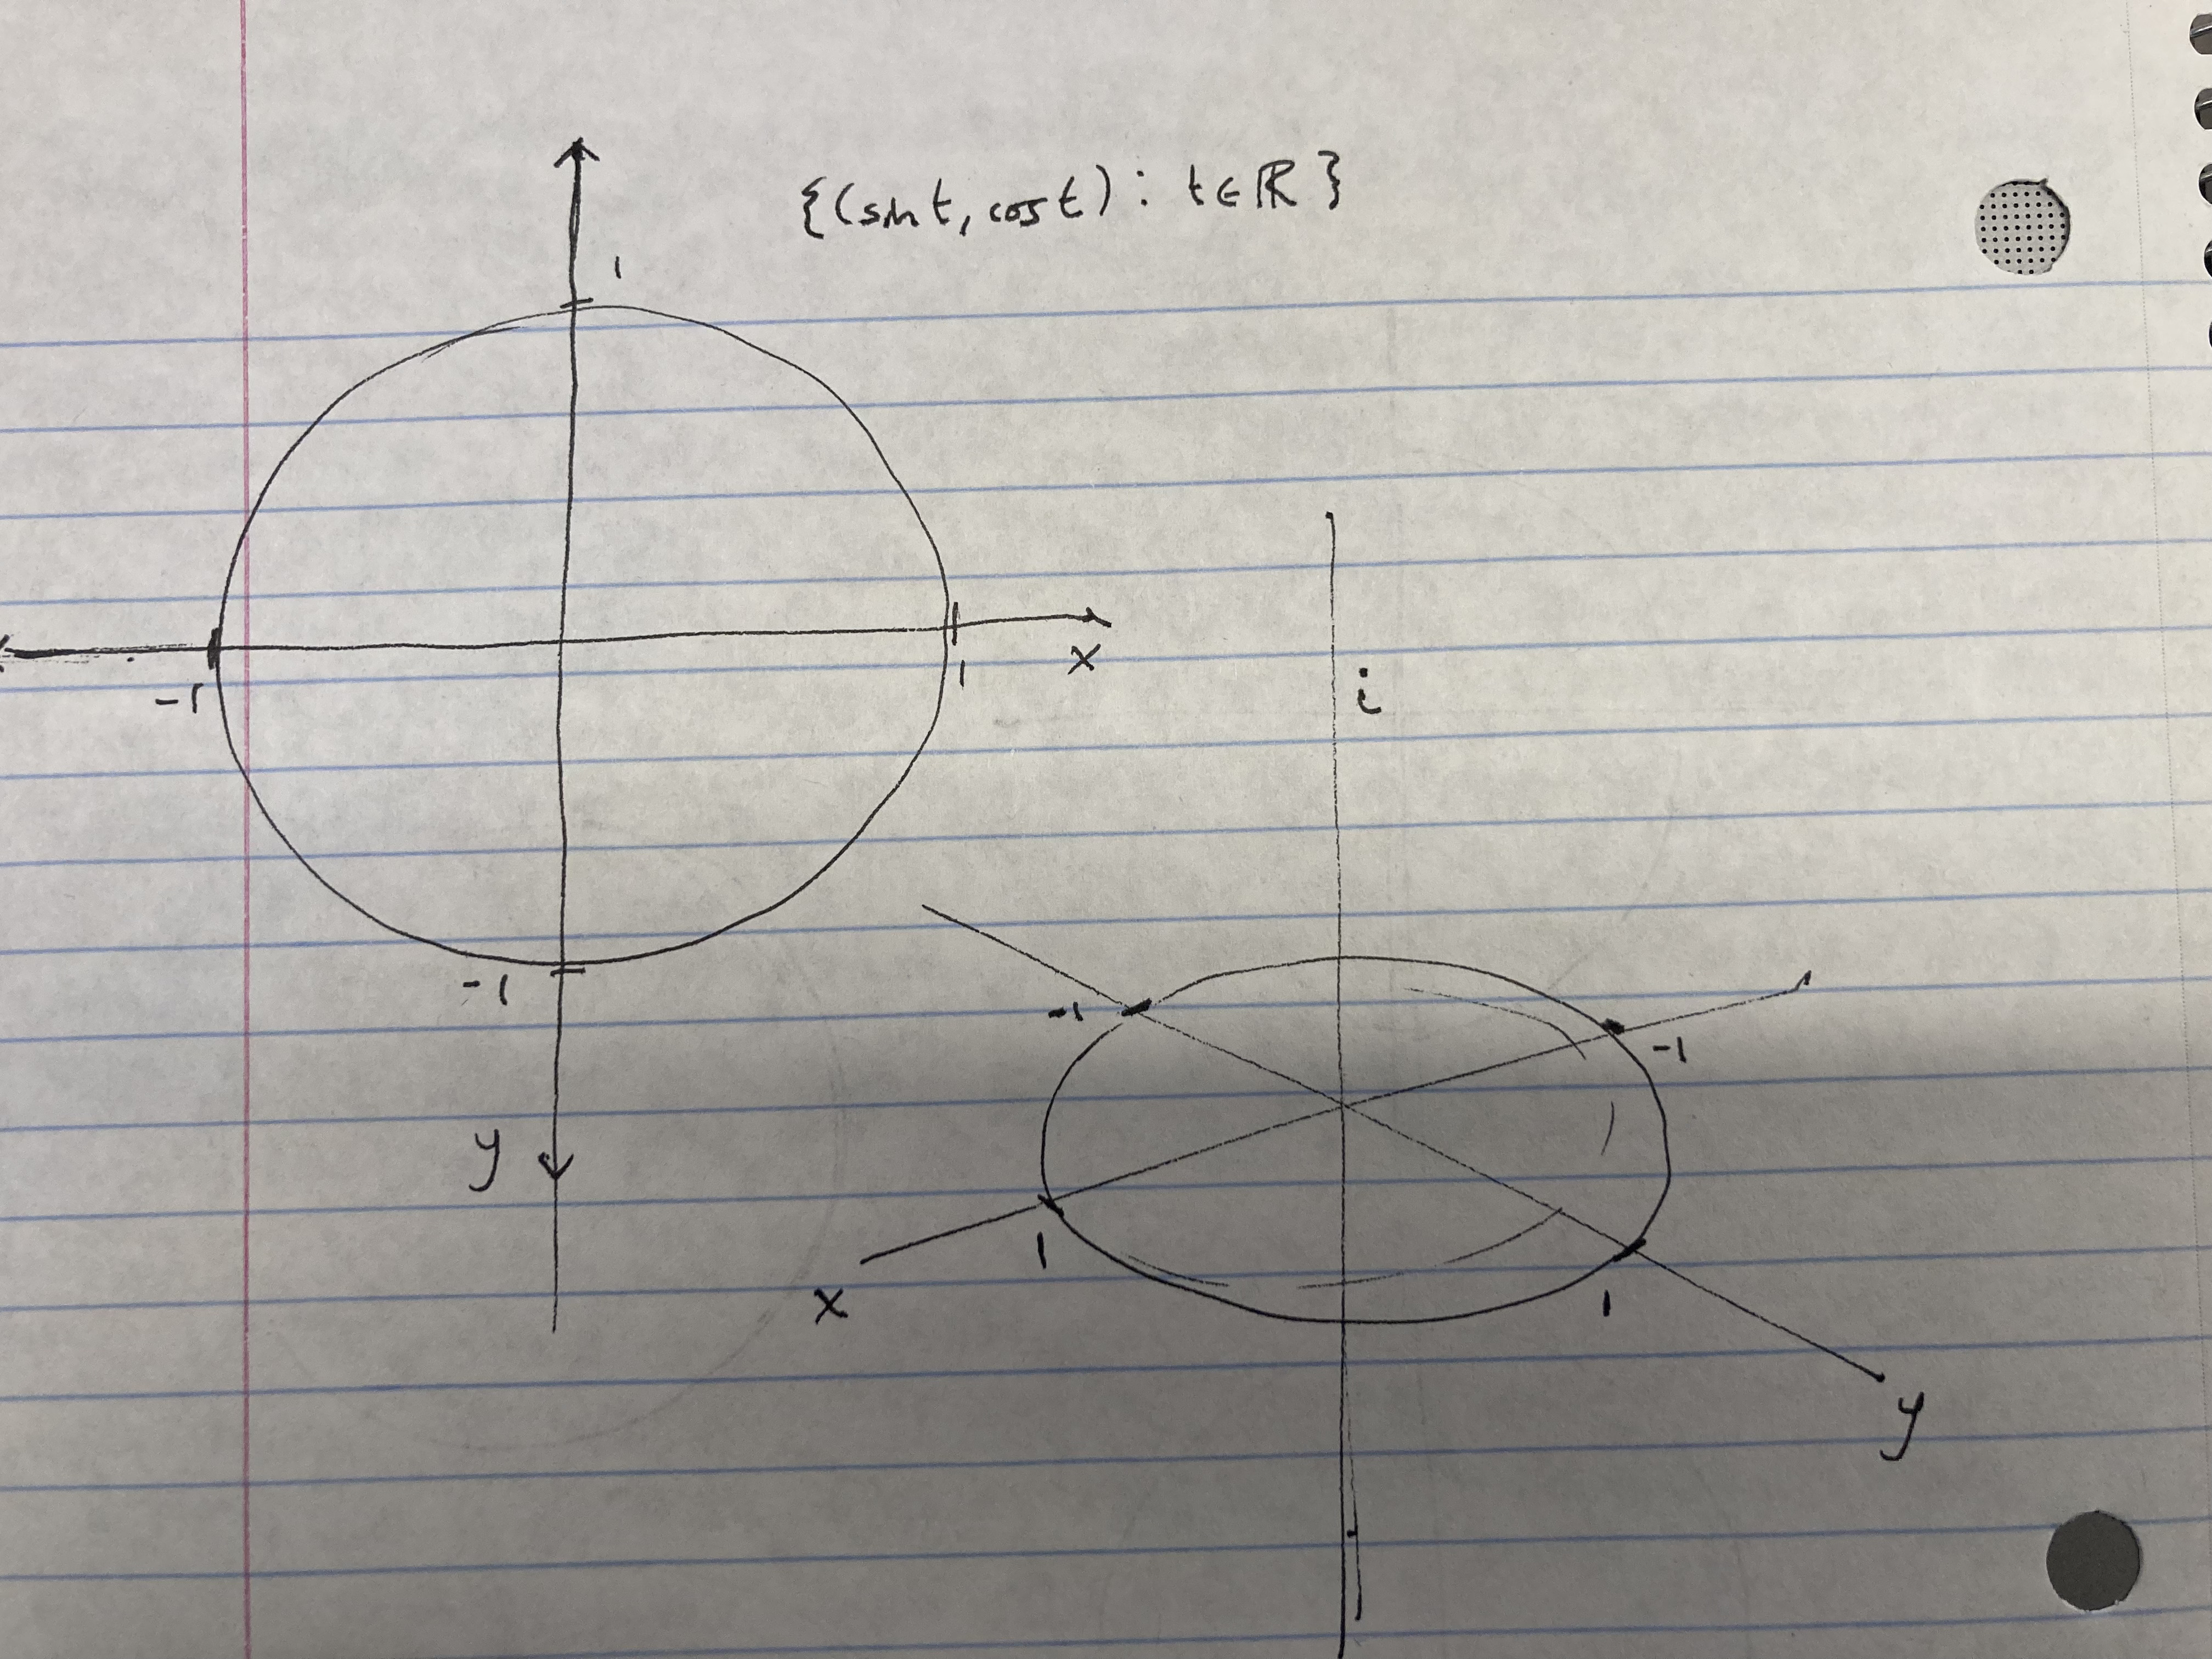
\includegraphics[scale=.07]{third}
                    \end{center}
            \end{proof}

        \item [(b)] $\{(x, y, z) : z > 0\} \subseteq \mathbb{A}^{3}_{\mathbb{R}}$
            \begin{proof}
                Suppose that $f \in I(\{(x, y, z) : z > 0\})$. If we look at $f(x, y, z)$ as a polynomial on one variable $z$, we conclude that $f = 0$ because $f \in V(\mathbb{A}^{1})$. So now we look at $f$ over $k[x, y, z]$. Since $f = 0$ over $k[x, y]$, then $f = 0$ over $k[x, y, z]$. So now we take $V(I(\{(x, y, z) : z > 0\})) = V(\{0\}) = \mathbb{A}^{3}_{\mathbb{R}}$. So the closure is the entire space. 
                    \begin{center}
                        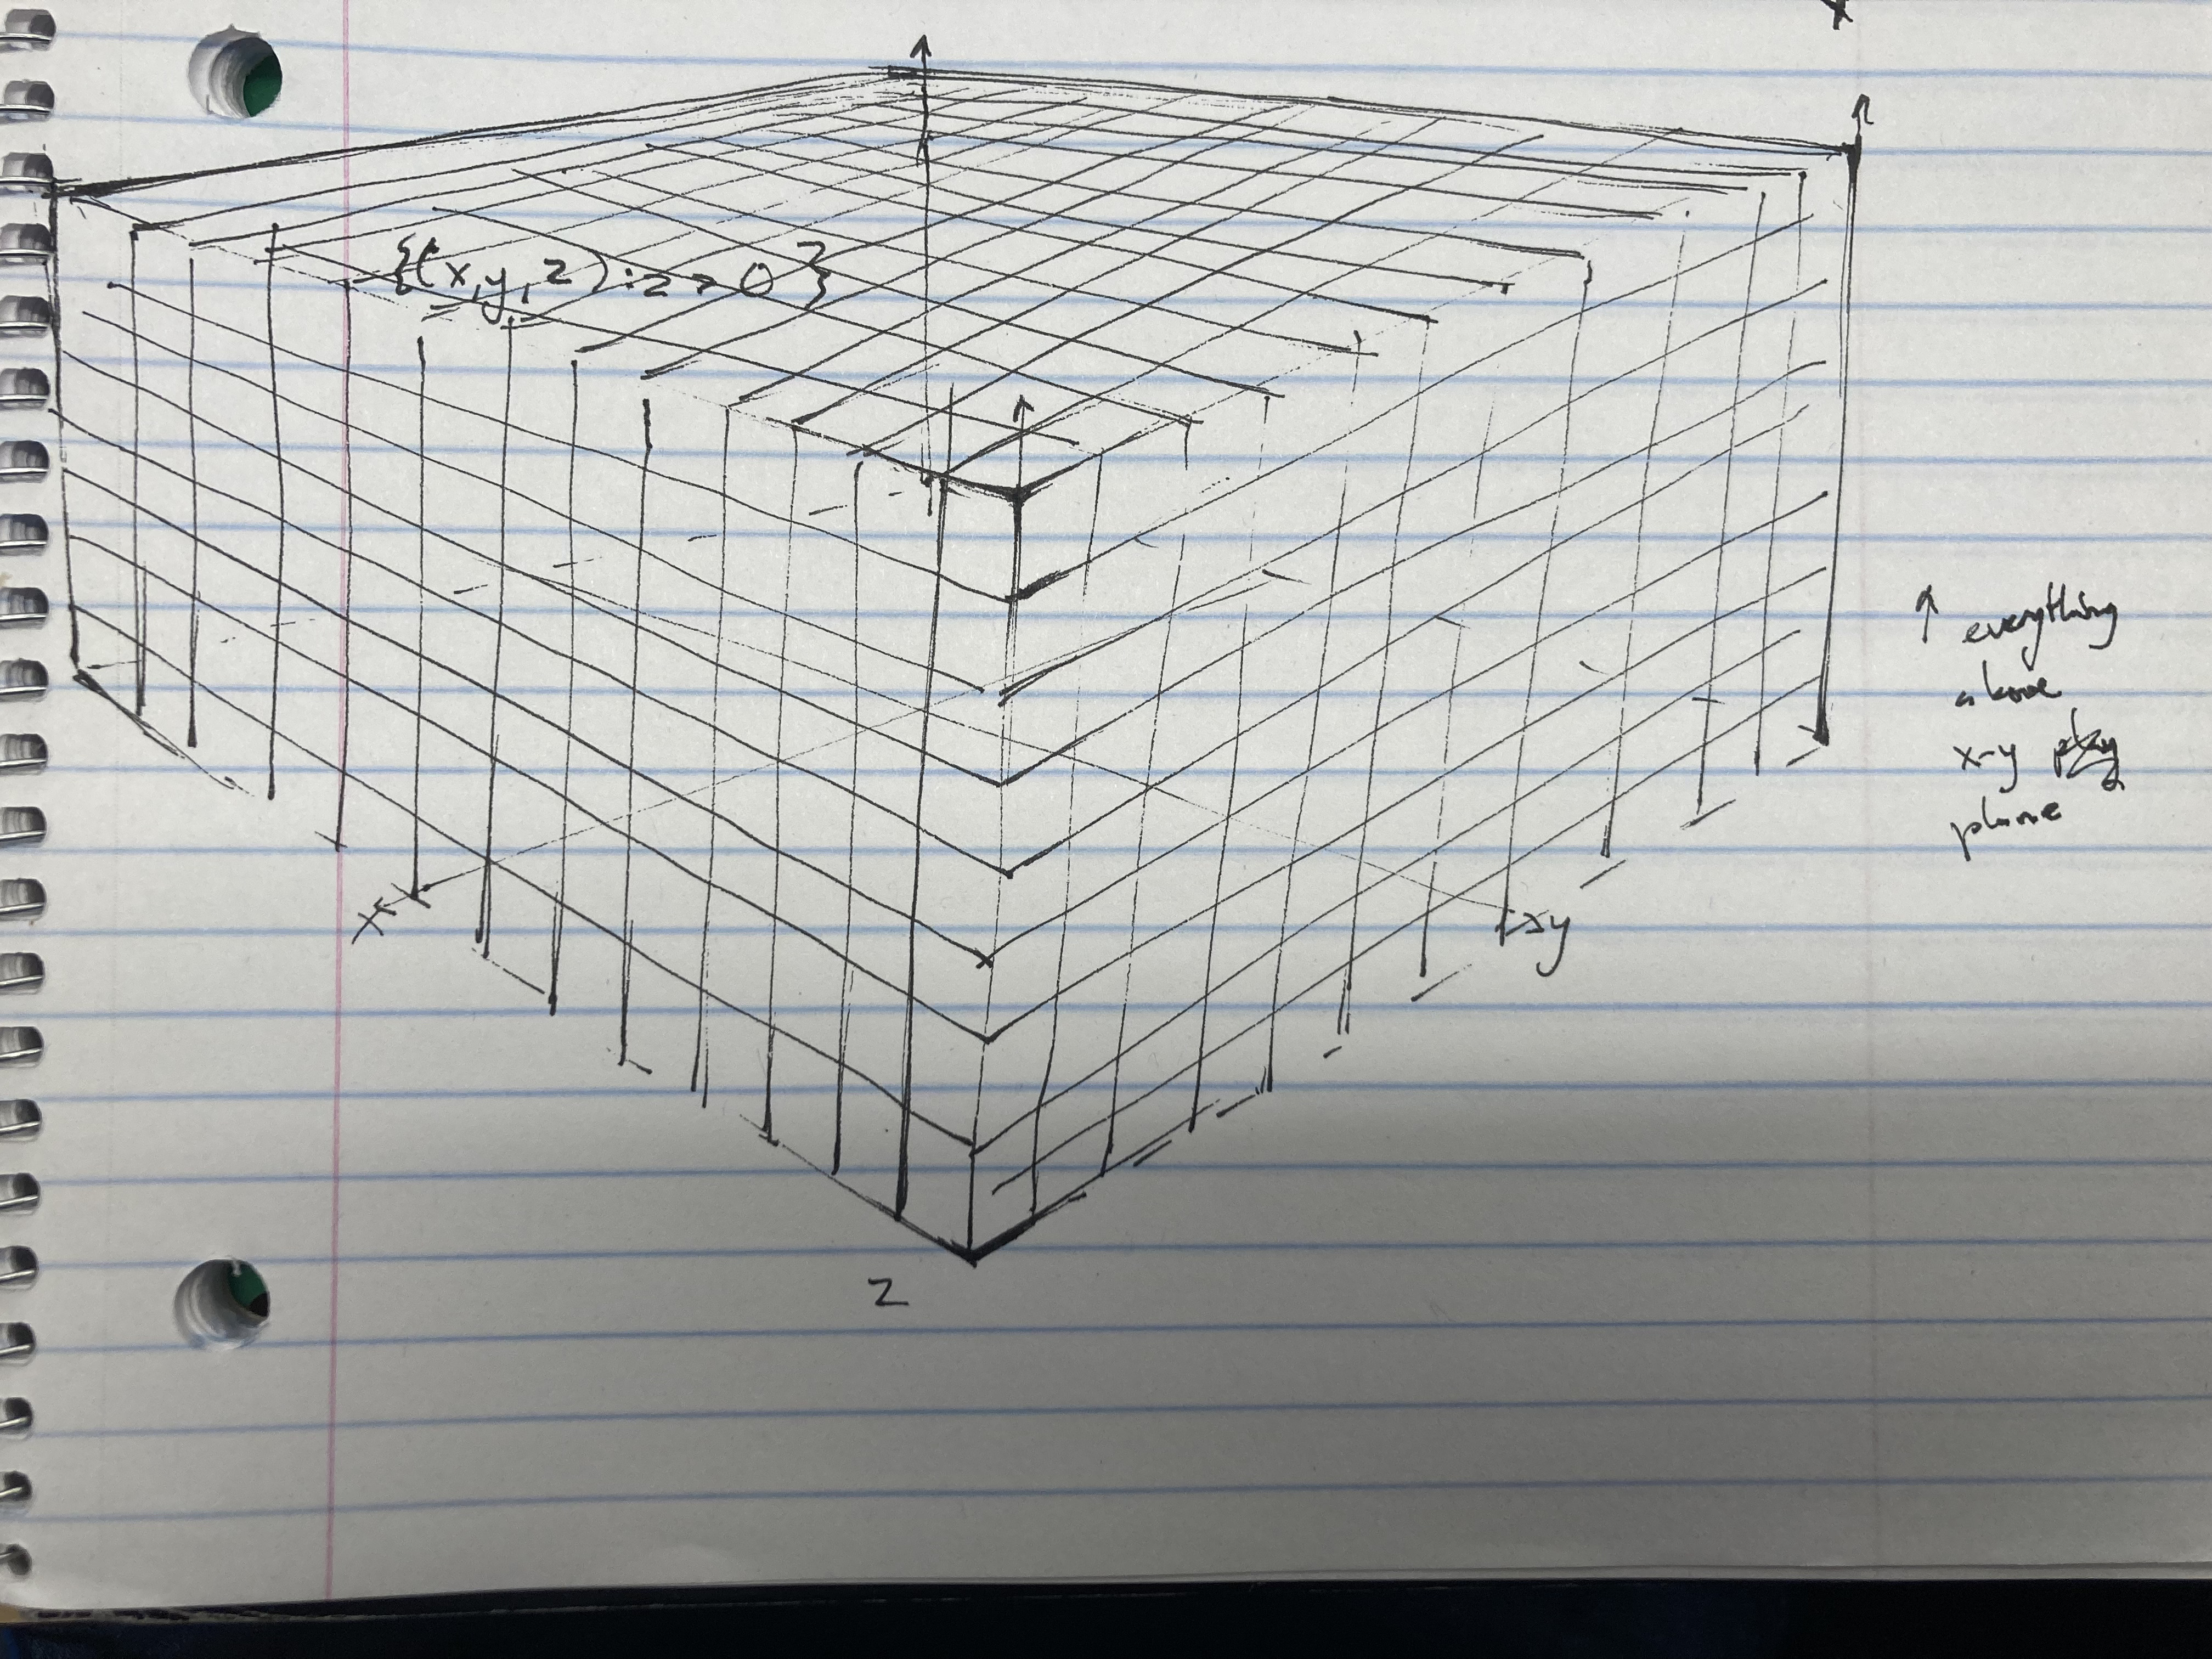
\includegraphics[scale=.07]{first}
                    \end{center}
            \end{proof}

        \item [(c)] $\{(x, y, z) : x = y \text{ or } x = z\} \subseteq \mathbb{A}^{3}_{\mathbb{C}}$
            \begin{proof}
                This set is an algebraic set because it is equivalent to $V(((x - z)(x - y)))$. If $(x, x, z) \in \{(x, y, z) : x = y \text{ or } x = z\}$, then we have for $f \in ((x - y)(x - z))$, $f((x, x, z)) = g(x, y, z) \cdot (x - x)(x - z) = 0$. The same case applies if $(x, y, x) \in \{...\}$ or in the case where $x = y$ and $x = z$. And points that lie in $V(((x - z)(x - y)))$ are killed by $f(x, y, z) = (x - z)(x - y)$ at the very least. So $0 = (x - z)(x - y)$. We are over an integral domain, $\mathbb{C}$. So either one has to be $0$. So $x = y$ or $x = z$ which shows the other inclusion. Since it is an algebraic set, it is equal to its closure.
                    \begin{center}
                        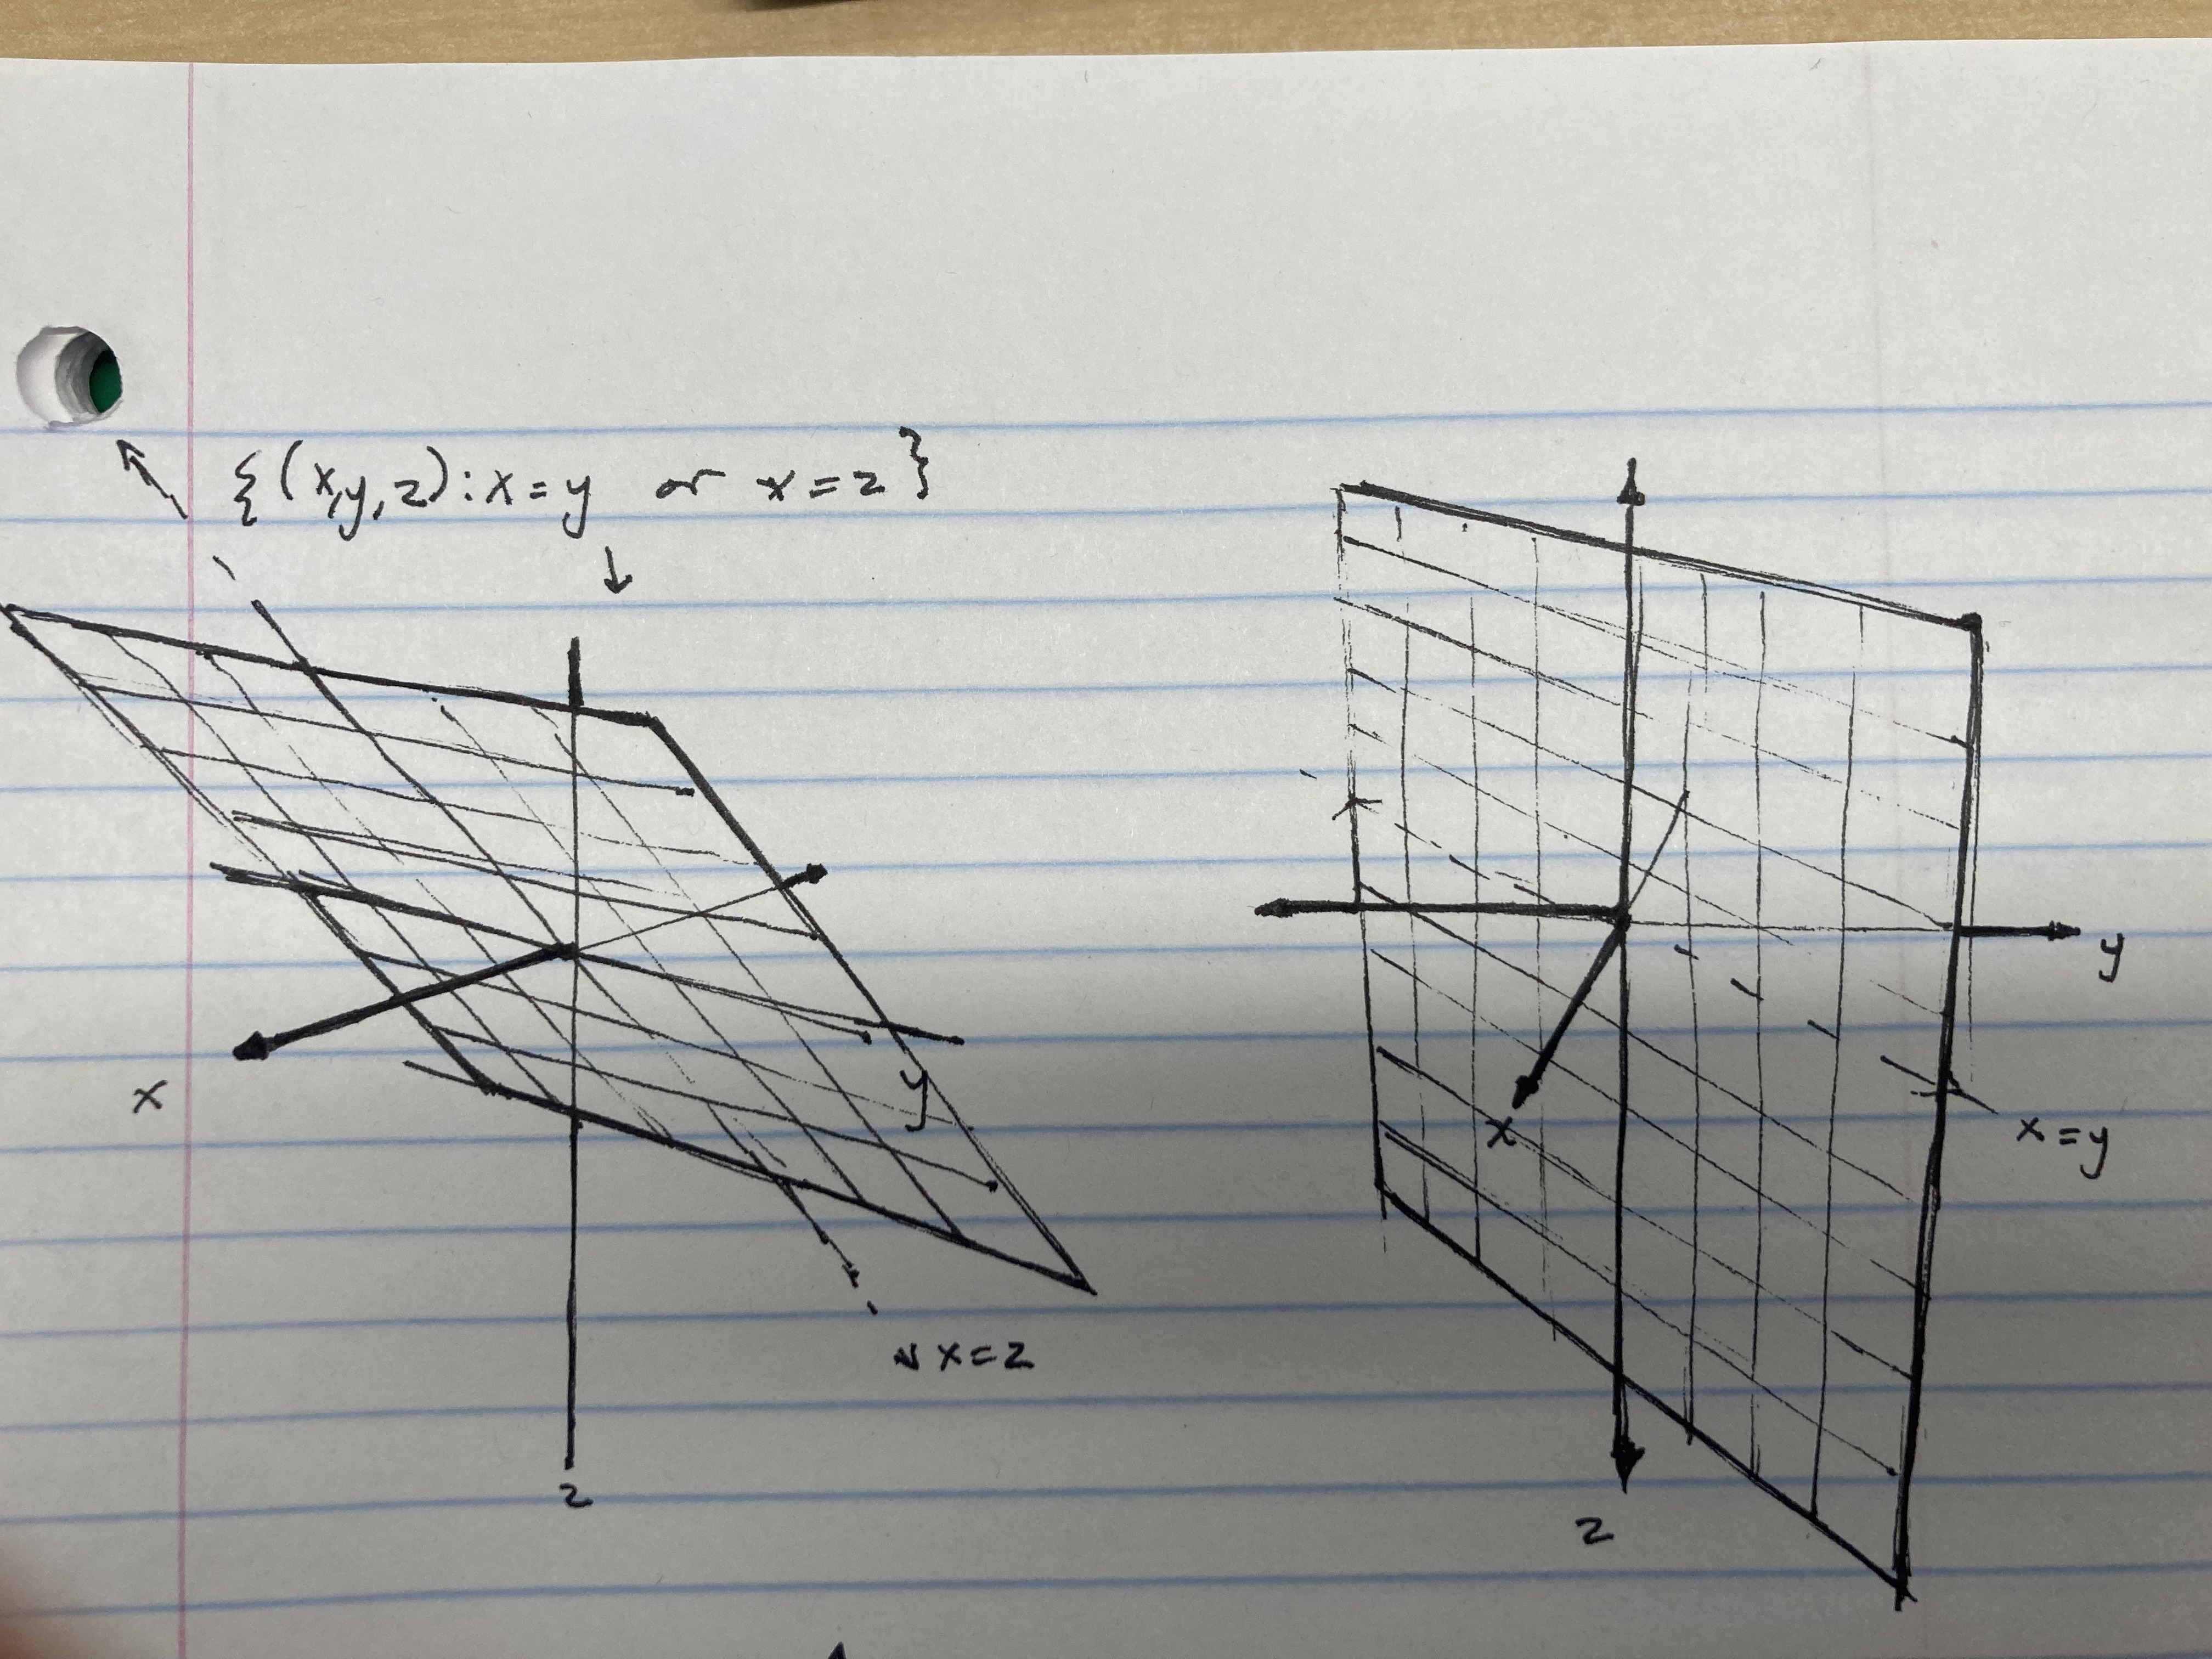
\includegraphics[scale=.07]{second}
                    \end{center}
            \end{proof}
    \end{itemize}

\textbf{Exercise 3}: Let $\varphi: \mathbb{A}^{2} \rightarrow \mathbb{A}^{2}$ be the morphism given by $(x, y) \mapsto (xy, y)$. 
    \begin{itemize}
        \item [(a)] Find the pullback map $\varphi : \Gamma(\mathbb{A}^{2}) \rightarrow \Gamma(\mathbb{A}^{2})$.
            \begin{proof}
                The pullback is 
                    \begin{equation*}
                        \varphi^{*} : k[x, y] \rightarrow k[u, v] 
                    \end{equation*}
                where
                    \begin{align*}
                        x &\mapsto uv \\
                        y &\mapsto v
                    \end{align*}
            \end{proof}

        \item [(b)] What is the image of $\varphi$? Is $\varphi$ dominant?
            \begin{proof}
                We have that 
                    \begin{equation*}
                        \Im{\varphi} = \{(xy, y) : x, y \in \mathbb{A}\}
                    \end{equation*}
                To see if $\varphi$ is dominant or not, we need to look at injectivity of $\varphi^{*}$. Suppose that 
                    \begin{equation*}
                        \varphi^{*}(f) = 0
                    \end{equation*}
                for some $f \in k[x, y]$. Then we need to show that $f = 0 \in k[x, y]$. Suppose that $f \neq 0$. Then we have that the degree of $f \geq 1$. So now we make the substitution on all $x$ in $f(x, y)$ as $x = uy$. We note that for a given term $cx^{k_{1}}y^{k_{2}}$ in $f$, we have:
                    \begin{equation*}
                        cu^{k_{1}}y^{k_{1} + k_{2}}
                    \end{equation*}
                and we find its inverse:
                    \begin{equation*}
                        cu^{k_{1}}y^{k_{1} + k_{2}} + g(uy, y) = 0
                    \end{equation*}
                The degree of $u$ tells us that $x$ has $k_{1}$ factors in $g(x, y)$. And that immediately tells us the degree of $y$. Finally, the coefficient and the fact that $k$ is an integral domain says that the inverse is just the negative version of the polynomial. So this means that substitution of $x = uy$ preserves additive inverses and therefore, $f(uy, y)$ is non-zero. Therefore, this contradicts the fact that $f(uv, v) = 0$. So $f = 0$ and $\varphi$ is dominant.
            \end{proof}

        \item [(c)] Although $\varphi$ is continuous, prove that the image is neither closed nor open in the Zariski topology. 
            \begin{proof}
                (Not Closed) We have that since $\varphi$ is dominant, 
                    \begin{equation*}
                        I(\varphi(\mathbb{A}^{2})) = I(\mathbb{A}^{2}) = 0
                    \end{equation*}
                and now the vanishing:
                    \begin{equation*}
                        V(I(\varphi(\mathbb{A}^{2}))) = \mathbb{A}^{2}
                    \end{equation*}
                but $\varphi(\mathbb{A}^{2}) \neq \mathbb{A}^{2}$ because the mapping is not surjective because we do not have points $(p_{1}, 0)$ for non-zero $p_{1} \in k$. This is because if $(a, b) \in \mathbb{A}^{2}$, then we require:
                    \begin{equation*}
                        \varphi(x, y) = (a, b)
                    \end{equation*}
                or 
                    \begin{equation*}
                        xy = a, y = b
                    \end{equation*}
                and therefore,  
                    \begin{equation*}
                        x = \dfrac{a}{b}
                    \end{equation*}
                which does not work when $y = b = 0$. So this tells us that $\varphi(\mathbb{A}^{2})$ is not closed because it is not equal to its closure. 

                (Not Open) By the previous part, we see that the elements not in $\varphi(\mathbb{A}^{2})$ are those of the form $(p_{1}, 0)$ for $p_{1} \neq 0 \in k$. So now we just need to show that the complement is not closed. Let
                    \begin{equation*}
                        Y = \varphi(\mathbb{A}^{2})^{c} = \{(p, 0): p \in k, p \neq 0\}
                    \end{equation*}
                Now the closure is just $\mathbb{A}^{1}$ because $Y \subseteq \mathbb{A}^{1}$ and is an infinite subset. But we know that the only algebraic subsets of $\mathbb{A}^{1}$ are either finite or $\mathbb{A}^{1}$ itself. So we have 
                    \begin{equation*}
                        V(I(Y)) = \mathbb{A}^{1} \neq Y
                    \end{equation*}
                So the complement is not closed and therefore, $\varphi(\mathbb{A}^{2})$ is not open.
            \end{proof}
    \end{itemize}

\textbf{Exercise 4}: A subset $A \subseteq X$ is called \textit{dense} if the closure of $A$ is all of $X$.
    \begin{itemize}
        \item [(a)] Suppose $f \in \Gamma(X)$ is a polynomial function and $A \subseteq X$ is a dense subset. Prove that if $f(P) = 0$ for all $P \in A$, then $f = 0 \in \Gamma(X)$.
            \begin{proof}
                This means that $f \in I(A)$. Now we have:
                    \begin{equation*}
                        V(I(A)) = X
                    \end{equation*}
                which comes from the fact that $A$ is dense and
                    \begin{equation*}
                        I(A) \subseteq I(V(I(A))) = I(X)
                    \end{equation*}
                But since $f \in I(A)$, we have $f\in I(X)$ and therefore, $f = 0 \in \Gamma(X)$.
            \end{proof}

        \item [(b)] Prove that $\varphi : X \rightarrow Y$ is dominant if and only if $\varphi(X)$ is dense in $Y$. (Recall that we defined $\varphi$ to be dominant if $I(\varphi(X)) = I(Y)$).
            \begin{proof}
                ($\rightarrow $) If $\varphi$ is dominant, we get
                    \begin{equation*}
                        I(\varphi(X)) = I(Y)
                    \end{equation*}
                and applying $V$ to both sides:
                    \begin{equation*}
                        V(I(\varphi(X))) = V(I(Y)) = Y \text{ since $Y$ is algebraic}
                    \end{equation*}
                so this means that the closure of $\varphi(X)$ is $Y$. So $\varphi(X)$ is dense in $Y$.

                ($\leftarrow $) Suppose that $\varphi(X)$ is dense in $Y$. Then that means
                    \begin{equation*}
                        V(I(\varphi(X))) = Y
                    \end{equation*}
                We can also see that 
                    \begin{equation*}
                        I(\varphi(X)) \subseteq I(V(I(\varphi(X)))) = I(Y)
                    \end{equation*}
                So we have proven one inclusion. Now we also have $\varphi(X) \subseteq Y$. By inclusion reversing, 
                    \begin{equation*}
                        I(\varphi(X)) \supseteq I(Y)
                    \end{equation*}
                So $I(\varphi(X)) = I(Y)$ which tells us that $\varphi : X \rightarrow Y$ is dominant.
            \end{proof}

        \item [(c)] Suppose $X$ is an algebraic set. Is the intersection of dense subsets always dense? Prove or give a counter example. (Do not assume that the subsets are open.)
            \begin{proof}
                Let $X = \mathbb{A}^{1}$ where $k = \mathbb{R}$. Now take the subsets $X_{1} = \{x \in \mathbb{A}^{1} : x > 0\}$ and $X_{2} = \{x \in \mathbb{A}^{1} : x < 0\}$. We notice that 
                    \begin{equation*}
                        V(I(X_{1})) = X \text{ and } V(I(X_{2})) = X
                    \end{equation*}
                because the algebraic sets of $\mathbb{A}^{1}$ are either finite or the entire field. But we observe that $X_{1} \cap X_{2} = \emptyset$ which is an algebraic set of $\mathbb{R}$. These are the vanishing of the irreducible quadratics of $\mathbb{R}[x]$. So the closure is $\emptyset \neq \mathbb{A}^{1}$.
            \end{proof}

        \item [(d)] Prove that if $X$ is an irreducible algebraic set and $U \subseteq X$ is a non-empty open subset, then $U$ is dense. 
            \begin{proof}
                Since $U$ is open, we have $X - U$ is closed. Then:
                    \begin{equation*}
                        X = U \cup X - U
                    \end{equation*}
                So now we just apply the vanishing and ideal operators:
                    \begin{equation*}
                        I(X) = I(U \cup X - U) = I(U) \cap I(X - U)
                    \end{equation*}
                and 
                    \begin{equation*}
                        V(I(X)) = V(I(U) \cap  I(X - U)) = V(I(U)) \cup V(I(X - U))
                    \end{equation*}
                Now since $X - U$ is algebraic, we know that its closure is itself, and the same goes for $X$:
                    \begin{equation*}
                        X = V(I(U)) \cup (X - U)
                    \end{equation*}
                But since $X$ is irreducible, it must be that either $X - U$ or $V(I(U))$ is a non-proper algebraic set. Since $U$ is non-empty, $X - U$ is not all of $X$, so it must be that $V(I(U)) = X$. This means that $U$ is dense in $X$.
            \end{proof}
    \end{itemize}

\textbf{Exercise 5}: Let $X \subseteq \mathbb{A}^{n}$ be an algebraic set, and let $f \in \Gamma(X)$ be a polynomial function. The \textit{graph} of $f$ is the set
    \begin{equation*}
        G(f) = \{(a_{1}, \ldots , a_{n}, a_{n + 1}) \in \mathbb{A}^{n + 1} : (a_{1}, \ldots , a_{n}) \in X \text{ and } a_{n + 1} = f(a_{1}, \ldots , a_{n})\}.
    \end{equation*}
        \begin{itemize}
            \item [(a)] Let $X = \mathbb{A}^{1}.$ Apply the definition above to describe the graph $x^{2} - 1 \in \Gamma(\mathbb{A}^{1}) = k[x]$ and draw a picture.
                \begin{answer}
                    By the definition, we have
                        \begin{equation*}
                            G(x^{2} - 1) = \{(a_{1}, a_{1}^{2} - 1) \in \mathbb{A}^{2}\}
                        \end{equation*}
                    Graphing this:
                            \begin{center}
                                \begin{tikzpicture}
                                    \begin{axis}[xmax=9,ymax=9, samples=50]
                                        \addplot[blue, thick] ({x}, {x^2 - 1});
                                    \end{axis}
                                \end{tikzpicture}
                            \end{center}
                \end{answer}

            \item [(b)] Prove that $G(f)$ is an algebraic set.
                \begin{proof}
                    We will show that $G(f) = V((x^{2} - 1 - y))$. Certainly, if $(a, a^{2} - 1) \in G(f)$, and $g \in (x^{2} - 1 - y)$,
                        \begin{equation*}
                            g(x, y) = h(x, y)(x^{2} - 1 - y)
                        \end{equation*}
                    so
                        \begin{equation*}
                            g(a, a^{2} - 1) = h(a, a^{2} - 1) (a^{2} - 1 - (a^{2} - 1)) = 0
                        \end{equation*}
                    which means $(a, a^{2} - 1) \in V((x^{2} - 1 - y))$. 

                    Now if $p = (x_{0}, y_{0}) \in V((x^{2} - 1 - y))$, then we require:
                        \begin{equation*}
                            x_{0}^{2} - 1 - y_{0} = 0
                        \end{equation*}
                    or
                        \begin{equation*}
                            y_{0} = x_{0}^{2} - 1
                        \end{equation*}
                    therefore, $p = (x_{0}, x_{0}^{2} - 1) \in G(f)$. So $G(f) = V(x^{2} - 1 - y)$.
                \end{proof}

            \item [(c)] Prove that $G(f)$ is isomorphic to $X$.
                \begin{proof}
                    We have a natural mapping from $\varphi : \mathbb{A}^{1} \rightarrow G(f)$ given by 
                        \begin{align*}
                            \varphi        &: \mathbb{A}^{1} \rightarrow G(f)  \\
                            \varphi(a)     &= (\varphi_{1}(a), \varphi_{2}(a)) \\
                            \varphi_{1}(a) &= a                                \\
                            \varphi_{2}(a) &= a^{2} - 1                          
                        \end{align*}
                    This is a polynomial map because $\varphi_{1}, \varphi_{2} \in k[x]$. Now we also have an inverse given by:
                        \begin{align*}
                            \varphi^{-1}       &: G(f) \rightarrow \mathbb{A}^{1} \\
                            \varphi^{-1}(a, b) &= a                                 
                        \end{align*}
                    which is a polynomial map. Now we just have to check that $\varphi\varphi^{-1} = id_{G(f)}$ and $\varphi^{-1}\varphi = id_{\mathbb{A}^{1}}$. 

                    ($\varphi\varphi^{-1} = id_{G(f)}$) We have:
                        \begin{align*}
                            \varphi\varphi^{-1}(a, a^{2} - 1) &= \varphi(a)                       \\
                                                              &= (\varphi_{1}(a), \varphi_{2}(a)) \\
                                                              &= (a, a^{2} - 1)                     
                        \end{align*}
                    ($\varphi^{-1}\varphi = id_{\mathbb{A}^{1}}$) We have:
                        \begin{align*}
                            \varphi^{-1}\varphi(a) &= \varphi^{-1}((\varphi_{1}(a), \varphi_{2}(a))) \\
                                                   &= \varphi^{-1}((a, a^{2} - 1))                   \\
                                                   &= a                                                
                        \end{align*}
                    which concludes the proof.
                \end{proof}
        \end{itemize}








\end{document}
